

Jennifer bought a box of Crunchy Grain cereal. The nutrition facts on the box state that a serving size of the cereal is $\frac{3}{4}$ cup and provides 210 calories, 50 of which are calories from fat. In addition, each serving of the cereal provides 180 milligrams of potassium, which is $5 \%$ of the daily allowance for adults. If $p$ percent of an adult's daily allowance of potassium is provided by $x$ servings of Crunchy Grain cereal per day, which of the following expresses $p$ in terms of $x$ ?\\
A. $p=0.5 x$\\
B. $p=5 x$\\
C. $p=(0.05)^{x}$\\
D. $p=(1.05)^{x}$

A school district is forming a committee to discuss plans for the construction of a new high school. Of those invited to join the committee, 15\% are parents of students, 45\% are teachers from the current high school, 25\% are school and district administrators, and the remaining 6 individuals are students. How many more teachers were invited to join the committee than school and district administrators?

\section*{ID: bd90f87e}
A table of the US minimum wage for 6 different years is shown below.

\begin{center}
\begin{tabular}{|c|c|}
\hline
Year & \begin{tabular}{c}
US \\
minimum \\
wage \\
(dollars \\
per hour) \\
\end{tabular} \\
\hline
1960 & 1.00 \\
\hline
1970 & 1.60 \\
\hline
1980 & 3.10 \\
\hline
1990 & 3.80 \\
\hline
2000 & 5.15 \\
\hline
2010 & 7.25 \\
\hline
\end{tabular}
\end{center}

What was the percent increase of the minimum wage from 1960 to 1970?\\
A. $30 \%$\\
B. $60 \%$\\
C. $62.5 \%$\\
D. $120 \%$

\section*{ID: 0ea56bb2}
\begin{center}
\begin{tabular}{|c|c|}
\hline
Year & \begin{tabular}{c}
Subscriptions \\
sold \\
\end{tabular} \\
\hline
2012 & 5,600 \\
\hline
2013 & 5,880 \\
\hline
\end{tabular}
\end{center}

The manager of an online news service received the report above on the number of subscriptions sold by the service. The manager estimated that the percent increase from 2012 to 2013 would be double the percent increase from 2013 to 2014. How many subscriptions did the manager expect would be sold in 2014?\\
A. 6,020\\
B. 6,027\\
C. 6,440\\
D. 6,468\\
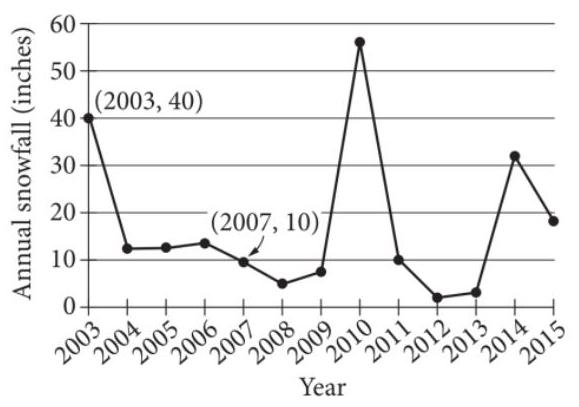
\includegraphics[max width=\textwidth, center]{2025_06_15_685e39be57606e31d5a9g-05}

The line graph shows the total amount of snow, in inches, recorded each year in Washington, DC, from 2003 to 2015. If $p \%$ is the percent decrease in the annual snowfall from 2003 to 2007, what is the value of $p$ ?

What percentage of 300 is 75 ?\\
A. $25 \%$\\
B. $50 \%$\\
C. $75 \%$\\
D. $225 \%$

The cost of a certain shirt is \$20 before a 5\% sales tax is added. What is the total cost, including sales tax, to purchase the shirt?\\
A. $\$ 20.05$\\
B. $\$ 20.50$\\
C. $\$ 21.00$\\
D. $\$ 25.00$

\section*{ID: 707db2d3}
For the finale of a TV show, viewers could use either social media or a text message to vote for their favorite of two contestants. The contestant receiving more than $50 \%$ of the vote won. An estimated $10 \%$ of the viewers voted, and $30 \%$ of the votes were cast on social media. Contestant 2 earned $70 \%$ of the votes cast using social media and $40 \%$ of the votes cast using a text message. Based on this information, which of the following is an accurate conclusion?\\
A. If all viewers had voted, Contestant 2 would have won.\\
B. Viewers voting by social media were likely to be younger than viewers voting by text message.\\
C. If all viewers who voted had voted by social media instead of by text message, Contestant 2 would have won.\\
D. Viewers voting by social media were more likely to prefer Contestant 2 than were viewers voting by text message.

\section*{ID: 63573fea}
During the first month of sales, a company sold 1,300,000 units of a certain type of smartphone. During the same month, $15 \%$ of the units sold were returned. If sales and the return rate remain the same for each of the next 5 months, about how many units of this smartphone will be returned to the company during this 6month period?\\
A. 195,000\\
B. 975,000\\
C. $1,170,000$\\
D. $6,630,000$

\section*{ID: 191d167b}
Last year, 200 students enrolled in an interior design program. This year, the number of students enrolled is $147 \%$ of last year's number. How many students are enrolled in the interior design program this year?\\
A. 247\\
B. 294\\
C. 347\\
D. 394







































\section*{ID: 949cd96b}
The length of the base of a certain parallelogram is $89 \%$ of the height of 
the parallelogram. Which expression represents the length of the base of the 
parallelogram, where $h$ is the height of the parallelogram?\\
A. $89 h$\\
B. $0.089 h$\\
C. $8.9 h$\\
D. 0.89 h

\section*{ID: 28c6bd8c}
Where Do People Get Most of Their Medical Information?

\begin{center}
\begin{tabular}{|l|c|}
\hline
\multicolumn{1}{|c|}{Source} & \begin{tabular}{c}
Percent of \\
those surveyed \\
\end{tabular} \\
\hline
Doctor & $63 \%$ \\
\hline
Internet & $13 \%$ \\
\hline
Magazines/brochures & $9 \%$ \\
\hline
Pharmacy & $6 \%$ \\
\hline
Television & $2 \%$ \\
\hline
Other/none of the above & $7 \%$ \\
\hline
\end{tabular}
\end{center}

The table above shows a summary of 1,200 responses to a survey question. Based on the table, how many of those surveyed get most of their medical information from either a doctor or the Internet?\\
A. 865\\
B. 887\\
C. 912\\
D. 926

Of 900,000 beads, 828,000 are silver. What percentage of the beads are silver?\\
A. $8 \%$\\
B. $36 \%$\\
C. $72 \%$\\
D. $92 \%$

\section*{ID: ba61d95f}
The population of Greenville increased by $7 \%$ from 2015 to 2016. If the 2016 population is $k$ times the 2015 population, what is the value of $k$ ?\\
A. 0.07\\
B. 0.7\\
C. 1.07\\
D. 1.7

\section*{ID: 8cbf1415}
In a group, $40 \%$ of the items are red. Of all the red items in the group, $30 \%$ also have stripes. What percentage of the items in the group are red with stripes?\\
A. $10 \%$\\
B. $12 \%$\\
C. $70 \%$\\
D. $75 \%$

A number $n$ is increased $6 \%$. If the result is 318 , what is the value of $n$ ?\\
A. 199\\
B. 299\\
C. 300\\
D. 337

\section*{ID: b2f6f17d}
A customer's monthly water bill was $\$ 75.74$. Due to a rate increase, her monthly bill is now $\$ 79.86$. To the nearest tenth of a percent, by what percent did the amount of the customer's water bill increase?\\
A. $4.1 \%$\\
B. $5.1 \%$\\
C. $5.2 \%$\\
D. $5.4 \%$

\section*{ID: 9c44f828}
There are a total of 840 seats in a school auditorium. During an assembly, students occupied $50 \%$ of the seats in the auditorium. How many seats did the students occupy during this assembly?\\
A. 25\\
B. 50\\
C. 420\\
D. 790

Isabel grows potatoes in her garden. This year, she harvested 760 potatoes and saved $10 \%$ of them to plant next year. How many of the harvested potatoes did Isabel save to plant next year?\\
A. 66\\
B. 76\\
C. 84\\
D. 86

According to the 2010 Census, the adult population aged 18 years or greater of the United States in 2010 was $234,564,071$. In 2010, a survey was conducted among a randomly chosen sample of adults aged 18 years or greater in the United States about their preference to live in a warm climate or a cool climate. The table below displays a summary of the survey results.

\begin{center}
\begin{tabular}{|l|l|l|l|l|}
\hline
\multicolumn{5}{|c|}{Climate Preferences} \\
\hline
 & Warm & Cool & No preference & Total \\
\hline
18-35 years old & 295 & 168 & 45 & 508 \\
\hline
36-50 years old & 246 & 123 & 41 & 410 \\
\hline
51-65 years old & 238 & 117 & 48 & 403 \\
\hline
Greater than 65 years old & 137 & 78 & 64 & 279 \\
\hline
Total & 916 & 486 & 198 & 1,600 \\
\hline
\end{tabular}
\end{center}

Which of the following is closest to the difference between the percentage of adults aged 18-50 years who responded "warm" and the percentage of adults aged 51 years or greater who responded "warm"?\\
A. $4 \%$\\
B. $5 \%$\\
C. $10 \%$\\
D. $18 \%$

\section*{ID: 7ed0d098}
Lani spent $15 \%$ of her 8 -hour workday in meetings. How many minutes of her workday did she spend in meetings?\\
A. 1.2\\
B. 15\\
C. 48\\
D. 72

The number $a$ is $70 \%$ less than the positive number $b$. The number $c$ is $60 \%$ greater than $a$. The number $c$ is how many times $b$ ?

The number $a$ is $110 \%$ greater than the number $b$. The number $b$ is $90 \%$ less than 47 . What is the value of $a$ ?

There are 170 blocks in a container. Of these blocks, $10 \%$ are green. How many blocks in the container are green?

\begin{center}
\begin{tabular}{|c|c|c|c|c|c|}
\hline
 & 1 Star & 2 Stars & 3 Stars & 4 Stars & Total \\
\hline
Employee A & 16 & 49 & 72 & 8 & 145 \\
\hline
Employee B & 4 & 10 & 22 & 34 & 70 \\
\hline
Employee C & 8 & 56 & 45 & 16 & 125 \\
\hline
Employee D & 22 & 42 & 84 & 12 & 160 \\
\hline
Total & 50 & 157 & 223 & 70 & 500 \\
\hline
\end{tabular}
\end{center}

A supervisor at a call center reviewed 500 calls taken by four employees and rated the employees' performance on each call on a scale from 1 star to 4 stars. The ratings for each employee are shown in the table above. According to the table, to the nearest whole percent, what percent of Employee A's calls received a rating of 1 star?\\
A. $3 \%$\\
B. $11 \%$\\
C. $16 \%$\\
D. $32 \%$

\section*{ID: 194ae3b1}
There were approximately 113,000 occupational therapy jobs in the United States in 2012. The Bureau of Labor Statistics has projected that this number will increase by $29 \%$ from 2012 to 2022. Of the following, which is closest to the number of occupational therapy jobs the bureau has projected for the United States in 2022?\\
A. 115,900\\
B. 116,300\\
C. 142,000\\
D. 145,800

\section*{ID: a8fabad0}
A waiter receives tips from each customer. On average, the tip is $15 \%$ of the customer's bill. At this rate, which of the following is closest to the tip the waiter can expect when a customer has a bill that is $\$ 78.20$ ?\\
A. $\$ 8.00$\\
B. $\$ 10.00$\\
C. $\$ 12.00$\\
D. $\$ 14.00$

The number $w$ is $110 \%$ greater than the number $z$. The number $z$ is $55 \%$ less than 50 . What is the value of $w$ ?

432 is $96 \%$ of what number?

\section*{ID: 7b731fc3}
What number is $40 \%$ greater than 115 ?

13 is $p \%$ of 25 . What is the value of $p$ ?

During a sale, the original prices of all the items in a clothing store have been reduced by $20 \%$. What is the sale price of a jacket with an original price of $\$ 50$ ?\\
A. $\$ 12$\\
B. $\$ 30$\\
C. $\$ 36$\\
D. $\$ 40$

\section*{ID: 3d73a58b}
A gift shop buys souvenirs at a wholesale price of 7.00 dollars each and resells them each at a retail price that is $290 \%$ of the wholesale price. At the end of the season, any remaining souvenirs are marked at a discounted price that is $80 \%$ off the retail price. What is the discounted price of each remaining souvenir, in dollars?

What is $10 \%$ of 370 ?\\
A. 27\\
B. 37\\
C. 333\\
D. 360

Thomas installed a new stove in his restaurant. At the time of installation, the stove had a value of $\$ 800$. Thomas estimates that each year the value of the stove will depreciate by $20 \%$ of the previous year's estimated value. What is the estimated value of the stove exactly 2 years after Thomas installed it?\\
A. $\$ 480$\\
B. $\$ 512$\\
C. $\$ 556$\\
D. $\$ 640$

\section*{ID: 6e4a60dd}
Rita's total bill at a restaurant was \$25.00, including tax. If she left a tip of 20\% of the total bill, what was the amount of the tip?\\
A. $\$ 3.50$\\
B. $\$ 4.00$\\
C. $\$ 4.50$\\
D. $\$ 5.00$

\section*{ID: 040f2a84}
The regular price of a shirt at a store is $\$ 11.70$. The sale price of the shirt is $80 \%$ less than the regular price, and the sale price is $30 \%$ greater than the store's cost for the shirt. What was the store's cost, in dollars, for the shirt? (Disregard the \$ sign when entering your answer. For example, if your answer is $\$ 4.97$, enter 4.97)

What number is 20\%\\
greater than 60 ?\\
A. 50\\
B. 72\\
C. 75\\
D. 132

Out of 300 seeds that were planted, $80 \%$ sprouted. How many of these seeds sprouted?

\section*{ID: 8213b1b3}
According to a set of standards, a certain type of substance can contain a maximum of $0.001 \%$ phosphorus by mass. If a sample of this substance has a mass of 140 grams, what is the maximum mass, in grams, of phosphorus the sample can contain to meet these standards?

\section*{ID: 34f8cd89}
$37 \%$ of the items in a box are green. Of those, $37 \%$ are also rectangular. Of the green rectangular items, $42 \%$ are also metal. Which of the following is closest to the percentage of the items in the box that are not rectangular green metal items?\\
A. $1.16 \%$\\
B. $57.50 \%$\\
C. $94.25 \%$\\
D. $98.84 \%$

The number $a$ is $60 \%$ greater than the positive number $b$. The number $c$ is $45 \%$ less than $a$. The number $c$ is how many times $b$ ?

\section*{ID: ad911622}
The value of a collectible comic book increased by $167 \%$ from the end of 2011 to the end of 2012 and then decreased by $16 \%$ from the end of 2012 to the end of 2013 . What was the net percentage increase in the value of the collectible comic book from the end of 2011 to the end of 2013?\\
A. $124.28 \%$\\
B. $140.28 \%$\\
C. $151.00 \%$\\
D. $209.72 \%$


